\documentclass[12pt]{article}

\usepackage[utf8]{inputenc}
\usepackage[T1]{fontenc}
\usepackage[spanish,mexico]{babel}
\usepackage{graphicx}
\usepackage[a4paper,margin=2.5cm]{geometry}
\usepackage{lmodern}
\usepackage{ragged2e}
\usepackage{array}
\usepackage{tabularx}

\begin{document}
\thispagestyle{empty}

\begin{center}

\includegraphics[width=1\textwidth]{encabezado_utvam.png}
\vspace{0.3cm}
{\small CÁLCULO IV}
\end{center}

\vspace{3cm}
\begin{center}
{\Large \textbf{Funciones de varias variables}}
\end{center}

\vspace{2.5cm}
\begin{center}
{\Large \textbf{Planos y superficies}}
\end{center}

\vspace{3cm}
\begin{center}
{\small \textbf{INTEGRANTES DEL EQUIPO:}}
\end{center}

\vspace{0.1cm}
\begin{center}
{\small 253110061 - López Lemus Glynnes Eileen}
\end{center}

\vspace{0.1cm}
\begin{center}
{\small 253110509 - Rodriguez Martinez Carlos Eduardo}
\end{center}

\vspace{0.1cm}
\begin{center}
{\small 253110366 - Salinas Sanchez Javier}
\end{center}

\vspace{0.1cm}
\begin{center}
{\small 253110017 - Roque Ubaldo Valeria}
\end{center}

\vspace{0.1cm}

\begin{center}
{\small \textbf{GRUPO: TID-401}}
\end{center}

\vspace{0.1cm}
\begin{center}
{\small \textbf{Docente: Rubén Ramírez Gómez}}
\end{center}

\vfill
\begin{flushright}
{\small SEPTIEMBRE, 2026}
\end{flushright}

\newpage

\begin{justfy}
{\Large \textbf{Actividad: El Escultor MAtematico 3D}}
\end{justfy}

\vspace{0.3cm}
\begin{justfy}
    \small \textbf{Anatomia Matematica:}
\end{justfy}

\begin{center}

\renewcommand{\arraystretch}{2}

\begin{tabular}{|p{3.2cm}|p{4.0cm}|p{4.0cm}|p{4.0cm}|}
\hline

\textbf{Parte del Objeto} &
\textbf{Superficie Elegida} &
\textbf{Ecuación Base} &
\textbf{Coordenadas del Centro (h,k,l)} \\

\hline
Cabeza &
Elipsoide &
$\displaystyle \frac{x^2}{a^2}+
\frac{y^2}{b^2}+
\frac{z^2}{c^2}=1$ &
$(0,0,5)$ \\

\hline
Torso &
Paraboloide elíptico &
$\displaystyle \frac{x^2}{a^2}+
\frac{y^2}{b^2}= z$ &
$(0,0,1.5)$ \\

\hline
Cuello &
Cilindro &
$\displaystyle x^2 + y^2 = r^2$ &
$(0,0,4.4)$ \\

\hline
Brazo izquierdo &
Cilindro &
$\displaystyle x^2 + y^2 = r^2$ &
$(-2,0,3)$ \\

\hline
Brazo derecho &
Cilindro &
$\displaystyle x^2 + y^2 = r^2$ &
$(2,0,3)$ \\

\hline
Pierna izquierda &
Cilindro &
$\displaystyle x^2 + y^2 = r^2$ &
$(-0.65,0,1)$ \\

\hline
Pierna derecha &
Cilindro &
$\displaystyle x^2 + y^2 = r^2$ &
$(0.65,0,1)$ \\
\hline
\end{tabular}
\end{center}

\vspace{0.5cm}
\begin{justfy}
    \small \textbf{Construccion (Esculpido):}
\end{justfy}

\vspace{1cm}
\begin{center}
    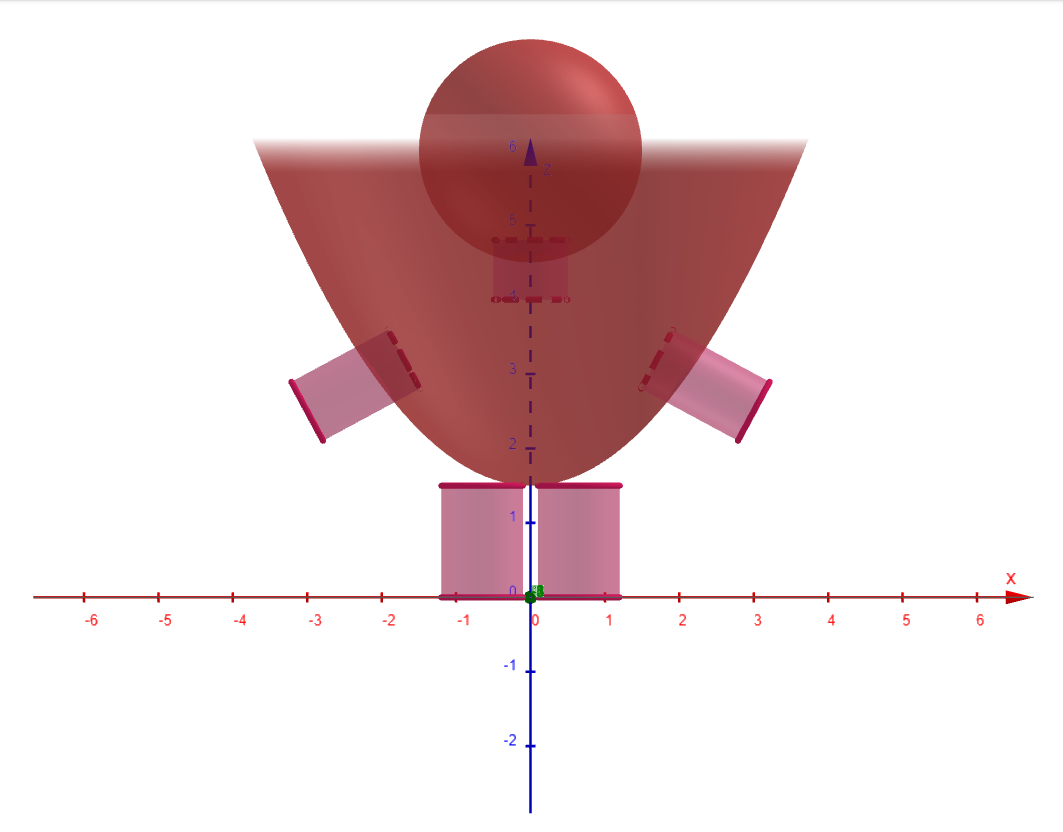
\includegraphics[width=0.45\textwidth]{Escultura geogebra.png}
    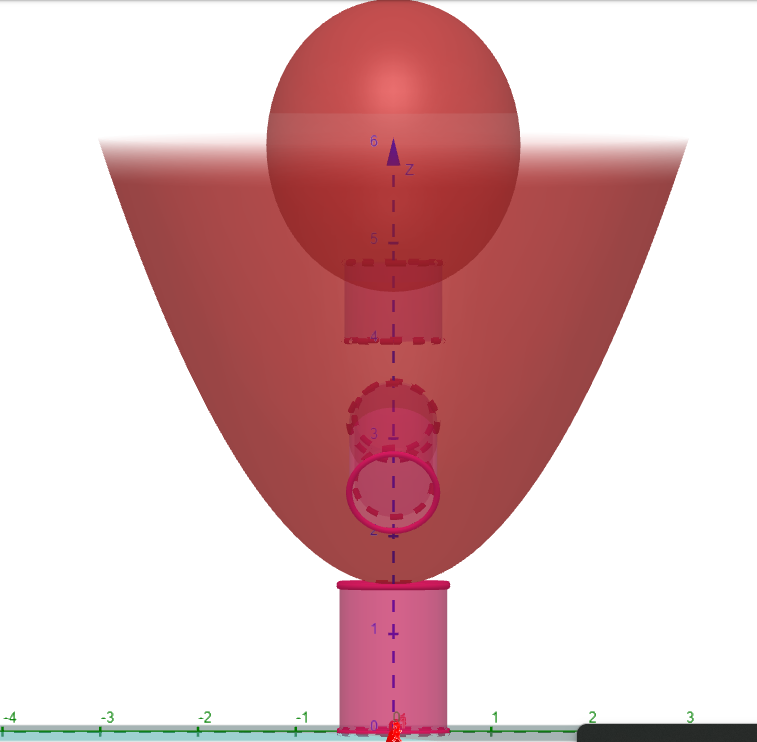
\includegraphics[width=0.45\textwidth]{Escultura geogebra 2.png}
    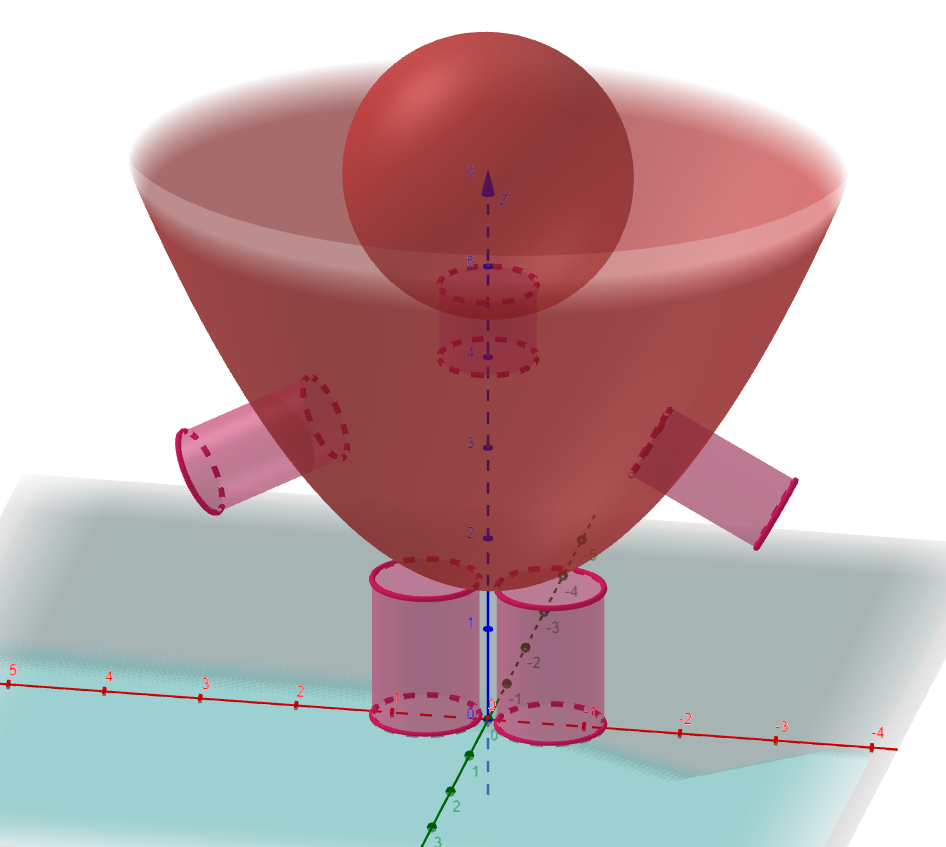
\includegraphics[width=0.50\textwidth]{Escultura geogebra 3.png}
\end{center}

\vspace{2cm}

\begin{justify}

\textbf{Análisis de Corte}

Realizamos el análisis de corte del torso en el que utilizamos un paraboloide elíptico.

Se creó un plano horizontal $z=k$ y se modificó el valor de $k$ mediante un deslizador y al caambiar la altura del plano, la estructura del torso cambio su tamaño. Al hacer esta interacción la curva resultante es una elipse y al aumentar k la elipse tambien aumenta de tamaño.
\end{justify}

\vspace{1cm}
\begin{center}
 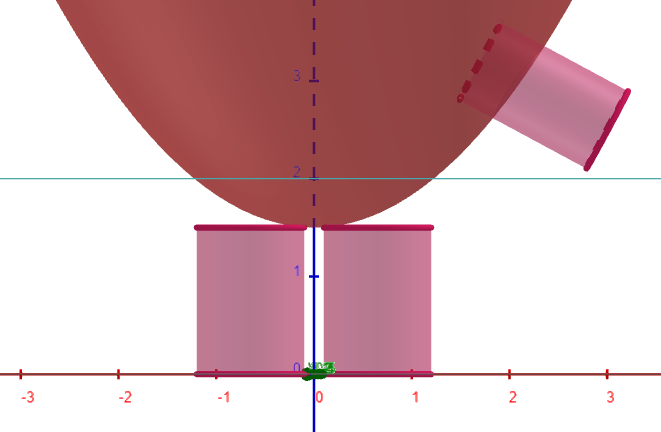
\includegraphics[width=0.75\textwidth]{Corte en estructura.png}
\end{center}
 
\end{document}
